\section{Исследование и построение решения задачи}
\label{sec:Section3} \index{Section3}

\subsection{Сбор данных для дальнейшего тестирования}

В данной работе генерация сигнатуры приложений рассматриваться не будет,
так как большинство современных приложений использует шифрование, а административные методы,
позволяющие дешифровать поступающий трафик, остаются за рамками данного исследования.
Однако были выбраны такие протоколы, которые покрывают все основные возможные проблемы,
возникающие при генерации сигнатур приложений, которые были описаны раннее.

Будут рассматриваться следующие протоколы: BitTorrent \cite{Bittorent}, DNS, FTP, HTTP, IMAP, POP3, SMTP.
HTTP - типичный представитель текстового протокола, который используется не только веб-приложениями,
но и в качестве туннеля.
FTP использует множественное подключение (как минимум двойное), при этом один канал является управляющим,
а через остальные происходит передача данных. DNS является представителем бинарного протокола, использующий UDP.
IMAP, SMTP, POP3 - почтовые протоколы c маленькими размерами пакетов.
BitTorrent - P2P протокол для кооперативного обмена файлами.

Исследуемый сетевой трафик снимался с кампусной сети ИСП РАН. Затем с помощью Wireshark \cite{Wireshark}
этот трафик был разбит по протоколам и результатом его работы были .pcap - файлы,
которые содержали в себе сессии определенного протокола, захваченные в течение исследуемого сетевого взаимодействия.
Пример выходного .pcap файла для HTTP можно увидеть на рис. \ref{wireshark}.

\begin{figure}[H]
    \begin{center}
        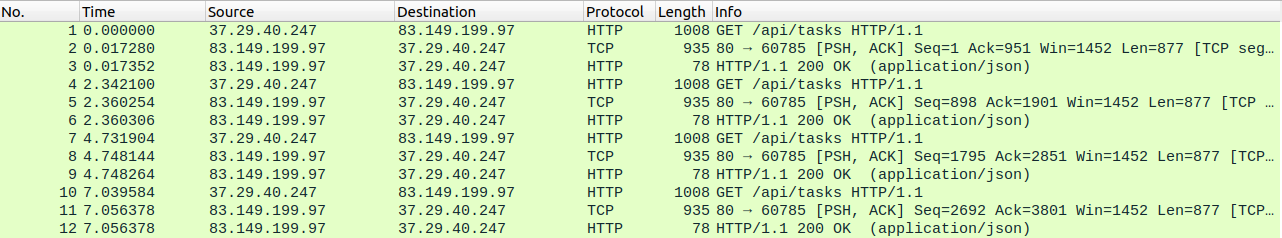
\includegraphics[width =\textwidth]{Wireshark.png}
        \caption{Пример работы Wireshark.}\label{wireshark}
    \end{center}
\end{figure}

В таблицах \ref{train_dataset} и \ref{test_dataset} представлены характеристики полученных данных для генерации сигнатур и их тестирования.
Классы протоколов дополнительно не балансировались.
В случае датасета генерации нас интересуют потоки, содержащие хотя бы 5 пакетов, так как в слишком коротких потоках сигнатуры может не быть.
Для тестирования был добавлен дополнительный класс <<other>>, в который включены
все остальные не рассматриваемые протоколы, и к которому классификатор будет относить все потоки, которым не соответствует ни одна сигнатура.

\begin{table}[ht!]
    \caption{Данные для генерации сигнатур.}
    \label{train_dataset}
    \centering
    \resizebox{0.9\columnwidth}{!}{
    \begin{tabular}{|c|c|c|c|c|c|c|}
        \hline
        Протокол   & \begin{tabular}[c]{@{}c@{}}Размер, \\ МБ\end{tabular} & \begin{tabular}[c]{@{}c@{}}Количество \\ пакетов\end{tabular} & \begin{tabular}[c]{@{}c@{}}Количество \\ потоков\end{tabular} &  \begin{tabular}[c]{@{}c@{}}Avg \\ bytes/pkt \end{tabular} &  \begin{tabular}[c]{@{}c@{}}Avg \\ pkts/stream \end{tabular} & \begin{tabular}[c]{@{}c@{}} Количество \\ потоков: \\ $\geq$ 5 pkts \end{tabular} \\ \hline
        bittorrent & 272,4      & 240159             & 708                & 1134                             & 339                                 & 214                                          \\ \hline
        dns        & 130,7      & 1283082            & 204150             & 102                              & 6                                   & 11027                                        \\ \hline
        ftp        & 0,86       & 16959              & 735                & 51                               & 23                                  & 725                                          \\ \hline
        http       & 1811,5     & 799062             & 13710              & 2268                             & 58                                  & 1500                                         \\ \hline
        imap       & 22,0       & 27702              & 66                 & 793                              & 419                                 & 65                                           \\ \hline
        pop        & 0,06       & 919                & 59                 & 64                               & 16                                  & 40                                           \\ \hline
        smtp       & 13,5       & 59121              & 1120               & 229                              & 53                                  & 799                                          \\ \hline
    \end{tabular}}
\end{table}

\begin{table}[ht!]
    \caption{Данные для тестирования сигнатур.}
    \label{test_dataset}
    \centering
    \resizebox{0.8\columnwidth}{!}{
    \begin{tabular}{|c|c|c|c|c|c|}
        \hline
        Протокол   & \begin{tabular}[c]{@{}c@{}}Размер, \\ МБ\end{tabular} & \begin{tabular}[c]{@{}c@{}}Количество \\ пакетов\end{tabular} & \begin{tabular}[c]{@{}c@{}}Количество \\ потоков\end{tabular} &  \begin{tabular}[c]{@{}c@{}}Avg \\ bytes/pkt \end{tabular} &  \begin{tabular}[c]{@{}c@{}}Avg \\ pkts/stream \end{tabular}\\ \hline
        bittorrent & 1,26       & 9409               & 876                & 133                              & 11                                  \\ \hline
        dns        & 53,3       & 664809             & 27800              & 80                               & 24                                  \\ \hline
        ftp        & 0,19       & 4000               & 294                & 48                               & 14                                  \\ \hline
        http       & 1494       & 406030             & 4607               & 3681                             & 88                                  \\ \hline
        imap       & 3,38       & 10587              & 143                & 320                              & 74                                  \\ \hline
        other      & 1119       & 1235122            & 18846              & 906                              & 66                                  \\ \hline
        pop        & 0,02       & 344                & 21                 & 58                               & 16                                  \\ \hline
        smtp       & 5,8        & 34428              & 1018               & 170                              & 34                                  \\ \hline
    \end{tabular}}
\end{table}

\subsection{Особенности при генерации сигнатур}

\begin{enumerate}
    \item
    Необходимо рассматривать только двунаправленные потоки, так как для генерации должны использоваться однородные потоки.
    Например, в случае HTTP набор общих подстрок для запросов и ответов разный.
    Поэтому необходимо либо уметь разделять потоки по направлениям и генерировать для каждого направления свою сигнатуру,
    либо не учитывать направление вовсе и генерировать общую сигнатуру.
    В первом случае, если не проводить семантический анализ протокола, то можно считать, что первый захваченный пакет
    в соединение идет от клиента к серверу, но это верно только для случая когда известно начало соединения.
    Это накладывает большое ограничение на выборку данных для генерации.
    Поэтому дальше будем рассматривать только двунаправленные потоки.

    \item
    Сигнатура обычно располагается в начале потока, поэтому не имеет смысла анализировать весь поток.
    Подбор константы первых анализируемых пакетов или байт полезной нагрузки является эвристическим.
    При этом привязку лучше делать по количеству пакетов из-за сильного разброса размеров пакетов разных протоколов,
    так как согласно \cite{park2008towards} сигнатура содержится в первых 10 пакетах потока.

    \item
    Необходимо ввести следующее эвристическое ограничение на сигнатуры, чтобы исключить тривиальные сигнатуры из рассмотрения:
    общая длина одной последовательности подстрок не меньше 8 символов
    и состоит хотя бы из 2 подстрок, каждая из которых не меньше 3 символов.

    \item
    Алгоритм AutoSig ввел дерево подстрок.
    Данная структура хороша тем, что увеличивает мощность получаемых сигнатур,
    это позволяет выделить несколько последовательностей подстрок, которые могут охватить те ситуация, в которых
    приложение имеет сильно разные потоки (например, поток управления и поток данных в FTP).
    Однако в том в виде, в котором это дерево представлено в работе \cite{ye2009autosig}, может получаться сильно избыточный набор сигнатур.
    Если узел является сигнатурным и не листом, то по свойству этого узла его набор потоков является строгим надмножеством
    наборов потоков любых других сигнатурных узлов, находящихся в его поддереве (например, листы, которые всегда являются сигнатурными),
    таким образом, любые пути из сигнатурных узлов поддерева являются избыточными, так как если нашлась последовательность подстрок
    соответствующая сигнатурному узлу из рассматриваемого поддерева,
    то найдётся в потоке и последовательность подстрок, соответствующая рассматриваемому узлу.
    При этом специфичность нашей сигнатуры за счёт этих сигнатурных узлов не увеличивается,
    так как для совпадения со сигнатурой достаточно совпадения последовательности подстрок,
    соответствующей нашему узлу, которая уже включена в другие.
    А значит поддерево можно удалить. Однако если не выполняется строгость надмножества, то последовательности строк
    поддерева не будут включаться друг в друга, а полнота покрытия потоков сохраниться,
    при этом вырастит специфичность (чем длиннее последовательность подстрок, тем специфичнее сигнатура).
    Именно поэтому при таком условии узел не становится сигнатурным.
\end{enumerate}

\subsection{Выбор алгоритма для автоматической генерации сигнатур}

В таблице \ref{methods} проведен сравнительный анализ рассмотренных ранее методов.

\begin{table}[ht]
    \caption{Сравнительный анализ методов автоматической генерации сигнатур.}
    \label{methods}
    \centering
    \resizebox{\columnwidth}{!}{
    \begin{tabular}{|c|c|c|c|}
        \hline
        Показатель\textbackslash{}Метод &
            LASER (LCS) &
            AutoSig &
            SigBox \\ \hline
        Тип сигнатуры &
            \begin{tabular}[c]{@{}c@{}}сигнатура пакета\\ (сигнатура потока)\end{tabular} &
            сигнатура потока &
            сигнатура потока \\ \hline
        Формат сигнатуры &
            \begin{tabular}[c]{@{}c@{}}последовательность \\ подстрок\end{tabular} &
            \begin{tabular}[c]{@{}c@{}}набор последовательностей \\ подстрок\end{tabular} &
            \begin{tabular}[c]{@{}c@{}}последовательность \\ подстрок\end{tabular} \\ \hline
        Тип ограничения &
            \begin{tabular}[c]{@{}c@{}}количество пакетов \\ (размер полезной нагрузки)\end{tabular} &
            размер полезной нагрузки &
            размер полезной нагрузки \\ \hline
        Агрегация потоков &
            не хранятся все потоки &
            хранятся все потоки &
            хранятся все потоки \\ \hline
        Сборка сессии &
            не требуется &
            требуется &
            не требуется \\ \hline
        Параметр поддержки &
            отсутствует &
            присутствует &
            \begin{tabular}[c]{@{}c@{}}не является \\ параметром алгоритма\end{tabular} \\ \hline
        \end{tabular}}
\end{table}

\textbf{Тип сигнатуры.} LASER извлекает наибольшую сигнатуру пакета, в то время как AutoSig и SigBox извлекают сигнатуры потоков.
Можно также применить шаг генерации алгоритма LASER - LCS, не только к пакету, но и ко всему потоку целиком, получив сигнатуру потока.

\textbf{Формат сигнатуры.} AutoSig в отличии от LASER и SigBox генерирует не одну последовательность подстрок,
а сразу несколько, используя дерево сигнатур.
Но как отмечалось уже раннее, это дерево сигнатур может быть избыточным.

\textbf{Тип ограничения.} Для алгоритмов AutoSig и SigBox используется ограничение по размеру полезной нагрузке потока,
т.е. потоки должен быть не меньше $n$-байт, но при этом использоваться будут только первые $n$-байт.
В свою очередь LASER использует аналогичное ограничение по числу пакетов.

\textbf{Агрегация потоков.} Для алгоритма LASER нет необходимости хранить все потоки одновременно,
так как при генерации одновременно используется не более 2 потоков.
А в случае AutoSig и SigBox необходимо хранить все потоки одновременно,
так как используется частотное распределение для построение сигнатур путём увеличения коротких последовательностей.

\textbf{Сборка сессии.} Несмотря на схожесть алгоритмов AutoSig и SigBox,
SigBox не требует сборки сессии из-за иерархического построения сигнатуры (содержимого -> пакета -> потока).
Для LASER сборка не требуется, так как он не работает на уровне потока.

\textbf{Параметр поддержки.} Этот параметр помогает бороться с шумами (потоки, которые сильно выбиваются по своему набору подстрок).
В LASER этот параметр не был заложен, его можно принимать константой равной $1,0$. В AutoSig этим параметром может выступать параметр <<S>> (пороговое значение слияния).
Этот параметр регулирует мощность набора сигнатур, если он равен $1,0$, то набор будет состоять не более, чем из 1 последовательности подстрок.
В SigBox этот параметр зафиксирован и равен $1,0$, таким образом
выходной сигнатурой SigBox тоже будет состоять не более, чем из 1 последовательности подстрок.

Таким образом, для дальнейших исследований был выбран алгоритм LASER, за свою простоту и не требовательность
к хранению всех потоков одновременно, что является важным параметром для интеграции в систему анализа сетевого трафика.
Также алгоритм LASER позволяет взять свой шаг генерации - алгоритм LCS, и попробовать получить сигнатуру потока.

\subsection{Реализация генератора и классификатора}

Был реализован генератор сигнатур с возможностью замены основного алгоритма генерации сигнатур.
В данной работе будет использоваться алгоритм LASER и его модификации.

Классификатор был также реализован с возможностью замены алгоритма сопоставления сигнатуры с полезной нагрузкой.
Он поддерживает сопоставление сигнатур пакетов, так и сигнатур потоков.

На описанных раннее данных были запущены генератор сигнатур и классификатор. Полученные результаты представлены на рис. \ref{matrix:laser} и в табл. \ref{report:laser}.

\begin{figure}[H]
    \begin{center}
        \includegraphics[width = 0.75\textwidth]{report/laser_no_filtered/Normalized_confusion_matrix.png}
        \caption{Матрица ошибок для алгоритма LASER.}
        \label{matrix:laser}
    \end{center}
\end{figure}

\begin{table}[ht!]
    \caption{Результаты классификации для алгоритма LASER.}
    \label{report:laser}
    \centering
    \resizebox{0.55\textwidth}{!}{
    \begin{tabular}{|c|c|c|c|c|}
        \hline
        protocol     & precision & recall & f1-score & support \\ \hline
        dns          & 0.93      & 1.00   & 0.97     & 27801   \\ \hline
        pop          & 0.80      & 0.19   & 0.31     & 21      \\ \hline
        smtp         & 0.94      & 0.92   & 0.93     & 1076    \\ \hline
        imap         & 1.00      & 0.57   & 0.72     & 175     \\ \hline
        bittorrent   & 0.92      & 0.97   & 0.95     & 886     \\ \hline
        ftp          & 0.99      & 0.97   & 0.98     & 295     \\ \hline
        http         & 0.99      & 0.94   & 0.96     & 4888    \\ \hline
        other        & 0.99      & 0.86   & 0.92     & 12094   \\ \hline
                     &           &        &          &         \\ \hline
        accuracy     &           &        & 0.95     & 47236   \\ \hline
        macro avg    & 0.95      & 0.80   & 0.84     & 47236   \\ \hline
        weighted avg & 0.95      & 0.95   & 0.95     & 47236   \\ \hline
    \end{tabular}}
\end{table}

Все протоколы, кроме POP3 и IMAP, отлично классифицируются: средневзвешенное значение F1-меры составило $0,95$.
Отклонения результата для POP3 и IMAP можно объяснить малым количеством потоков для генерации сигнатур этих протоколов.
Из матрицы ошибок также можно увидеть, что сигнатуры DNS не являются специфичными.

Рассмотрим среднее количество потоков необходимое для генерации сигнатуры.
Согласно табл. \ref{signature-generation} наибольшее среднее количество потоков, потребовавшееся для генерации 1 сигнатуры, равно $80,5$ для FTP.
Это объясняется тем, что в FTP есть два разных потока: управления и данных,
и алгоритм LASER не способен генерировать сигнатуру для сильно разных потоков в отличии от AutoSig и SigBox,
поэтому генератор дожидается того момента, пока не придут потоки одного типа.
Малое количество сигнатур POP3 объясняется малым количеством потоков в начальных данных. Все остальные результаты согласуются с \cite{santosautomatic}.

\begin{table}[ht!]
    \caption{Среднее количество потоков необходимое для генерации сигнатуры.}
    \label{signature-generation}
    \centering
    \resizebox{0.6\textwidth}{!}{
        \begin{tabular}{|c|c|c|}
        \hline
        Протокол & Количество сигнатур & \begin{tabular}[c]{@{}c@{}}Среднее количество \\ потоков на 1 сигнатуру\end{tabular} \\ \hline
        bittorrent & 51                  & 4,1                                       \\ \hline
        dns        & 682                 & 16,1                                      \\ \hline
        ftp        & 9                   & 80,5                                      \\ \hline
        http       & 145                 & 10,3                                      \\ \hline
        imap       & 10                  & 6,5                                       \\ \hline
        pop        & 2                   & 20,0                                      \\ \hline
        smtp       & 167                 & 4,8                                       \\ \hline
        \end{tabular}}
\end{table}

\subsection{Влияние постобработки на результаты классификации}

Стоит отметить большое количество сигнатур DNS, которые естественным образом перестают быть специфичными и являются избыточными.
Необходимо выполнять постобработку для генерируемых сигнатур.

Постобработка будет состоять из следующих шагов:

\begin{enumerate}
    \item удаление дубликатов
    \item удаление надмножеств
\end{enumerate}

Первый шаг очень естественный. На втором шаге предлагается удалить надмножества.
Согласно раннее описанному недостатку введенному дереву сигнатур в AutoSig, если представлять набор последовательностей подстрок
(все сигнатуры можно объединить в один набор)
в виде дерева, то не имеет смысла иметь в наборе сигнатуры, от корня до узлов которых на пути встречаются другие сигнатурные узлы.
Если эта сигнатура была найдена в полезной нагрузке, то это значит, что и любая её часть была найдена в полезной нагрузке.
Удаляя такие сигнатуры сильно уменьшается количество сигнатур в наборе, при этом качество классификации не изменяется.

Если бы удалялись подмножества, т.е. оставлялись самые специфичные сигнатуры, то количество сигнатур в наборе изменялось меньше,
а качество классификации меняется (обычно) в худшую сторону, так как остаются сигнатуры специфичные для малой подвыборки потоков.


Результаты постобработки приведены в табл. \ref{post-processing}.

\begin{table}[ht!]
    \caption{Количество сигнатур после постобработки.}
    \label{post-processing}
    \centering
    \resizebox{0.45\textwidth}{!}{
    \begin{tabular}{|c|cc|cc|}
    \hline
    Протокол & \multicolumn{2}{c|}{\begin{tabular}[c]{@{}c@{}}Количество\\ сигнатур\end{tabular}} & \multicolumn{2}{c|}{Избыточность} \\ \cline{2-5}
               & \multicolumn{1}{c|}{Было} & Стало & \multicolumn{1}{c|}{Было} & Стало \\ \hline
    bittorrent & \multicolumn{1}{c|}{51}   & 7     & \multicolumn{1}{c|}{0.53} & 0.53  \\ \hline
    dns        & \multicolumn{1}{c|}{682}  & 64    & \multicolumn{1}{c|}{0.99} & 0.99  \\ \hline
    ftp        & \multicolumn{1}{c|}{9}    & 8     & \multicolumn{1}{c|}{0.98} & 0.98  \\ \hline
    http       & \multicolumn{1}{c|}{145}  & 47    & \multicolumn{1}{c|}{1.00} & 1.00  \\ \hline
    imap       & \multicolumn{1}{c|}{10}   & 4     & \multicolumn{1}{c|}{1.00} & 0.79  \\ \hline
    pop        & \multicolumn{1}{c|}{2}    & 1     & \multicolumn{1}{c|}{1.00} & 0.00  \\ \hline
    smtp       & \multicolumn{1}{c|}{167}  & 26    & \multicolumn{1}{c|}{0.99} & 0.99  \\ \hline
    \end{tabular}}
\end{table}

Приблизительно половина всех удаленных сигнатур была дубликатами, остальные - надмножеством.
Можно увидеть, что такая простая постобработка не помогла сильно уменьшить избыточность сигнатур, т.е. найти минимальное покрывающее множество.
Поэтому в дальнейших исследованиях планируется рассмотреть более мощные методы.

\subsection{Влияние сборки сессии на результаты классификации}

Теперь рассмотрим модификацию алгоритма LASER. Шагом генерации сигнатуры в нем является алгоритм LCS, который выделяет общие подстроки у двух потоков байт.
В оригинальном алгоритме шаг генерации применялся к пакетам, но теперь будем применять к потоку.

Будут исследоваться следующие две модификации:

\begin{enumerate}
    \item c частичной сборкой сессии
    \item с полной сборкой сессии
\end{enumerate}

Под частичной сборкой сессии понимается, что полезная нагрузка пакетов собирается в один поток байт до первого пакета другого направления.
Для UDP полезная нагрузка просто конкатенируется, а для TCP также восстанавливаться правильный порядок пакетов.

На рис. \ref{matrix:laser_reasm} и в табл. \ref{report:laser_reasm} представлены результаты для частичной сборки сессии.
Результаты получились аналогичными оригинальному алгоритму,
небольшое отклонение связано с изменением значения числа <<пакетов>> для рассмотрения.
Оно было изменено таким образом, чтобы число потоков удовлетворяющему требованию на размер потока, осталось примерно таким же.

\begin{figure}[H]
    \begin{center}
        \includegraphics[width = 0.75\textwidth]{report/laser_reasm/Normalized_confusion_matrix.png}
        \caption{Матрица ошибок для алгоритма LASER с частичной сборкой сессии.}
        \label{matrix:laser_reasm}
    \end{center}
\end{figure}

\begin{table}[th!]
    \caption{Результаты классификации для алгоритма LASER с частичной сборкой сессии.}
    \label{report:laser_reasm}
    \centering
    \resizebox{0.55\textwidth}{!}{
    \begin{tabular}{|c|c|c|c|c|}
    \hline
    protocol     & precision & recall & f1-score & support \\ \hline
    dns          & 0.92      & 0.96   & 0.94     & 10565   \\ \hline
    pop          & 0.67      & 0.19   & 0.30     &    21   \\ \hline
    smtp         & 0.78      & 0.94   & 0.85     &  1464   \\ \hline
    imap         & 0.91      & 0.48   & 0.62     &   189   \\ \hline
    bittorrent   & 0.95      & 0.97   & 0.96     &   853   \\ \hline
    ftp          & 0.99      & 0.99   & 0.99     &   288   \\ \hline
    http         & 1.00      & 0.94   & 0.97     &  4890   \\ \hline
    other        & 0.88      & 0.81   & 0.85     &  4804   \\ \hline
                 &           &        &          &         \\ \hline
    accuracy     &           &        & 0.92     & 23074   \\ \hline
    macro avg    & 0.89      & 0.79   & 0.81     & 23074   \\ \hline
    weighted avg & 0.92      & 0.92   & 0.92     & 23074   \\ \hline
    \end{tabular}}
\end{table}

На рис. \ref{plt:lcs} представлены результаты для случая полной сборки сессии.
Как можно видеть, выделенные сигнатуры получились не специфичными.
Связано это с привязкой уже к размеру рассматриваемой полезной нагрузки.
Значение равное 1 КБ было выбрано согласно \cite{ye2009autosig}.
Положение сигнатуры все же привязано к определенным номерам пакетов,
а из-за разного распределения размеров для протоколов, нельзя использовать одно значение размера полезной нагрузки для всех протоколов.

\begin{figure}[H]
    \begin{center}
        \includegraphics[width = 0.75\textwidth]{report/lcs/Normalized_confusion_matrix.png}
        \caption{Матрица ошибок для алгоритма LASER с полной сборкой сессии.}
        \label{plt:lcs}
    \end{center}
\end{figure}

\newpage
